% !TeX encoding = UTF-8
% !TeX spellcheck = fr_FR

\documentclass{article}
\usepackage[utf8]{inputenc}
\usepackage[french]{babel}
\usepackage[T1]{fontenc}
%====================== PACKAGES ======================
%pour gérer les positionnement d'images
\usepackage{float}
\usepackage{amsmath,amssymb,amsthm}
\usepackage{graphicx}
\usepackage[colorinlistoftodos]{todonotes}
\usepackage{url}
%pour les informations sur un document compilé en PDF et l\section{}es liens externes / internes
\usepackage{hyperref}
%pour la mise en page des tableaux
\usepackage{array}
\usepackage{tabularx}
\usepackage[thinlines]{easytable}
%pour utiliser \floatbarrier
%\usepackage{placeins}
%\usepackage{floatrow}
%espacement entre les lignes
\usepackage{setspace}
%modifier la mise en page de l'abstract
\usepackage{fancyhdr}
\usepackage{abstract}
%police et mise en page (marges) du document

\usepackage{pdfpages}

\usepackage{csquotes}
%Code source
\usepackage{listingsutf8}

\usepackage[top=2cm, bottom=2cm, left=2cm, right=2cm]{geometry}
%Pour les galerie d'images
\usepackage{subfig}

% Glossaire
\usepackage[xindy]{glossaries}	% Ensures that all acronyms are defined once
\makeglossaries

\pagestyle{fancy}
\headheight=14.62pt

%% Mise en page des théorèmes, lemme etc...
\theoremstyle{plain}
\newtheorem{thm}{Théorème}[section]
\newtheorem{lemme}[thm]{Lemme}
\newtheorem{prop}[thm]{Proposition}
\newtheorem*{cor}{Corollaire}
\theoremstyle{definition}
\newtheorem{defn}{Définition}[section]
\newtheorem{conj}{Conjecture}[section]
\newtheorem{exmp}{Exemple}[section]
\theoremstyle{remark}
\newtheorem*{rem}{Remarque}
\newtheorem*{note}{Note}
\newtheorem{case}{Cas particulier}

\renewcommand{\floatpagefraction}{0.95}
\renewcommand{\textfraction}{0.05}

%====================== INFORMATION PDF======================

\hypersetup{												% Information sur le document
	pdfauthor = {Fati CHEN},								% Auteurs
	pdftitle = {Ouvertures et Finales d'Eternity II},		% Titre du document
	pdfsubject = {Rapport de Projet},						% Sujet
	pdfkeywords = {Eternity II, rapport de projet, LIRMM},	% Mots-clefs
	pdfstartview={FitH}										% ajuste la page à la largueur de l'écran
	pdfcreator = {MikTeX},									% Logiciel qui a crée le document
	pdfproducer = {Eternithug}}								% Société avec produit le logiciel


%======================== DEBUT DU DOCUMENT ========================
\begin{document}

	%__ Listes
	\renewcommand{\labelitemi}{$\bullet$}
	\renewcommand{\labelitemii}{$\cdot$}
	\renewcommand{\labelitemiii}{$\diamond$}
	\renewcommand{\labelitemiv}{$\ast$}

	%__ régler l'espacement entre les lignes
	\newcommand{\HRule}{\rule{\linewidth}{0.5mm}}

	%========================= Debut du texte =========================

	\pagenumbering{Alph}

\begin{titlepage}
	\begin{center}
	
	% Upper part of the page. The '~' is needed because only works if a paragraph has started.
	%\includegraphics[width=0.35\textwidth]{./logo}~\\[1cm]
	
	\textsc{\LARGE Faculté des Sciences\\
		Université de Montpellier\\
		Lirmm\\} \ \\[1.5cm]
	
	\textsc{\Large }\\[0.5cm]
	
	% Title
	\HRule \\[0.4cm]
	
	{\huge \bfseries Rapport de stage\\
	Ouvertures et finales d'Eternity II\\[0.4cm] }
	
	\HRule \\[1.5cm]
	
	% Author and supervisor
	\begin{minipage}{0.4\textwidth}
		\begin{flushleft} \large
			\emph{Auteurs:}\\
				Fati \textsc{Chen}\\
		\end{flushleft}
	\end{minipage}
	\begin{minipage}{0.4\textwidth}
		\begin{flushright} \large
			\emph{Référent:} \\
				Eric \textsc{Bourreau}
		\end{flushright}
	\end{minipage}
	
	\vfill
	\thispagestyle{empty}

	% Bottom of the page
	{\large \today}
	\end{center}
\end{titlepage}

\pagenumbering{arabic}

	\section{Introduction}

	Les puzzles et casses-têtes nous ont toujours passionnés, pour faire passer le temps ou pour se mettre des défis. Eternity II est un de ces jeux où le principe peux être compris par tous, mais pourtant sa résolution est extrêmement complexe. Ce genre de paradigme est à l'heure actuelle l'un des problèmes mathématiques qui régit notre monde, car la plupart des systèmes informatiques et méthodes de chiffrement reposent sur ce genre de problème (simple à faire mais pourtant trouver la solution ne l'est pas).

	Eternity II n'est résoluble à l'heure actuelle qu'en testant toutes les combinaisons (bruteforce). Ce qui nous fait poser une question importante, comment, avec l'augmentation exponentielle des données et des nouvelles technologies, sommes nous réduit à utiliser une méthode aussi simple.
	Par extension, est-il plus efficace d'accumuler des données afin de le résoudre plutôt qu'essayer d'accélérer la résolution basique.

	Dans un premier temps, nous verrons les origines du jeu, la difficulté à laquelle nous sommes confrontés et l'état de l'art des méthodes de résolutions.

	Ensuite, nous présenterons la problématique, ce qui à déjà tout au long de l'année et l'approche initiale du problème.

	Pour conclure, les résultats et réflexions qui peuvent en être tirés.

	Par ailleurs, ce compte rendu comporte un manuel d'utilisation et un manuel technique fourni, car les application développées, ou tout du moins leur logique est destinée à être réutilisés ou améliorés.


	\newpage
	% !TeX root = main.tex
\section{Eternity II}
	\subsection{Les origines}
	--- [réel]
	
	Eternity II est le fier successeur de Eternity.
	
	La première version sortie en 1999, était composée de 159 pièces de différentes formes, cependant ces formes peuvent être décomposés en formes de trianges equilatéraux (ou leur moitié) qui devaient être placés sur un plateau octogonal. 
	
	\begin{figure}[H]
		\minipage{0.65\textwidth}
		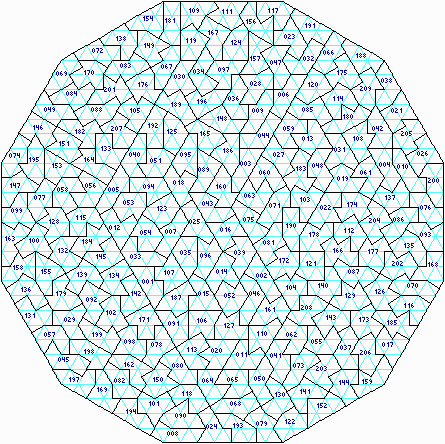
\includegraphics[width=\linewidth]{images/eternity_1.jpg}
		\caption{Eternity I}\label{fig:eternity_1}
		\endminipage\hfill
		\minipage{0.33\textwidth}
		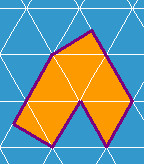
\includegraphics[width=\linewidth]{images/eternity_1_piece.jpg}
		\caption{Forme d'une pièce d'EternityI}\label{fig:eternity_1_piece}
		\endminipage\hfill
	\end{figure}

	Son point faible se trouvaient dans la disposition de ces pièces sur le plateau : il était possible de précalculer des régions, puis de les comparer entre eux afin d'en dégager une solution.
	De cette facon, le puzzle fut résolu en à peine un an (contrairement aux 3 ans prévus par le créateur), par deux mathématiciens, qui ont ainsi empoché la récompense s'élevant à $1000000\pounds$.
	
	Après cet \enquote{echec}, Christopher Monckton, le créateur d'Eternity, décide en 2008 de sortir une deuxième version, bien plus complexe avec à la clé $2000000$\textdollar pour celui qui arriverait à la résoudre au bout de deux ans.
	
	\begin{figure}[H]
		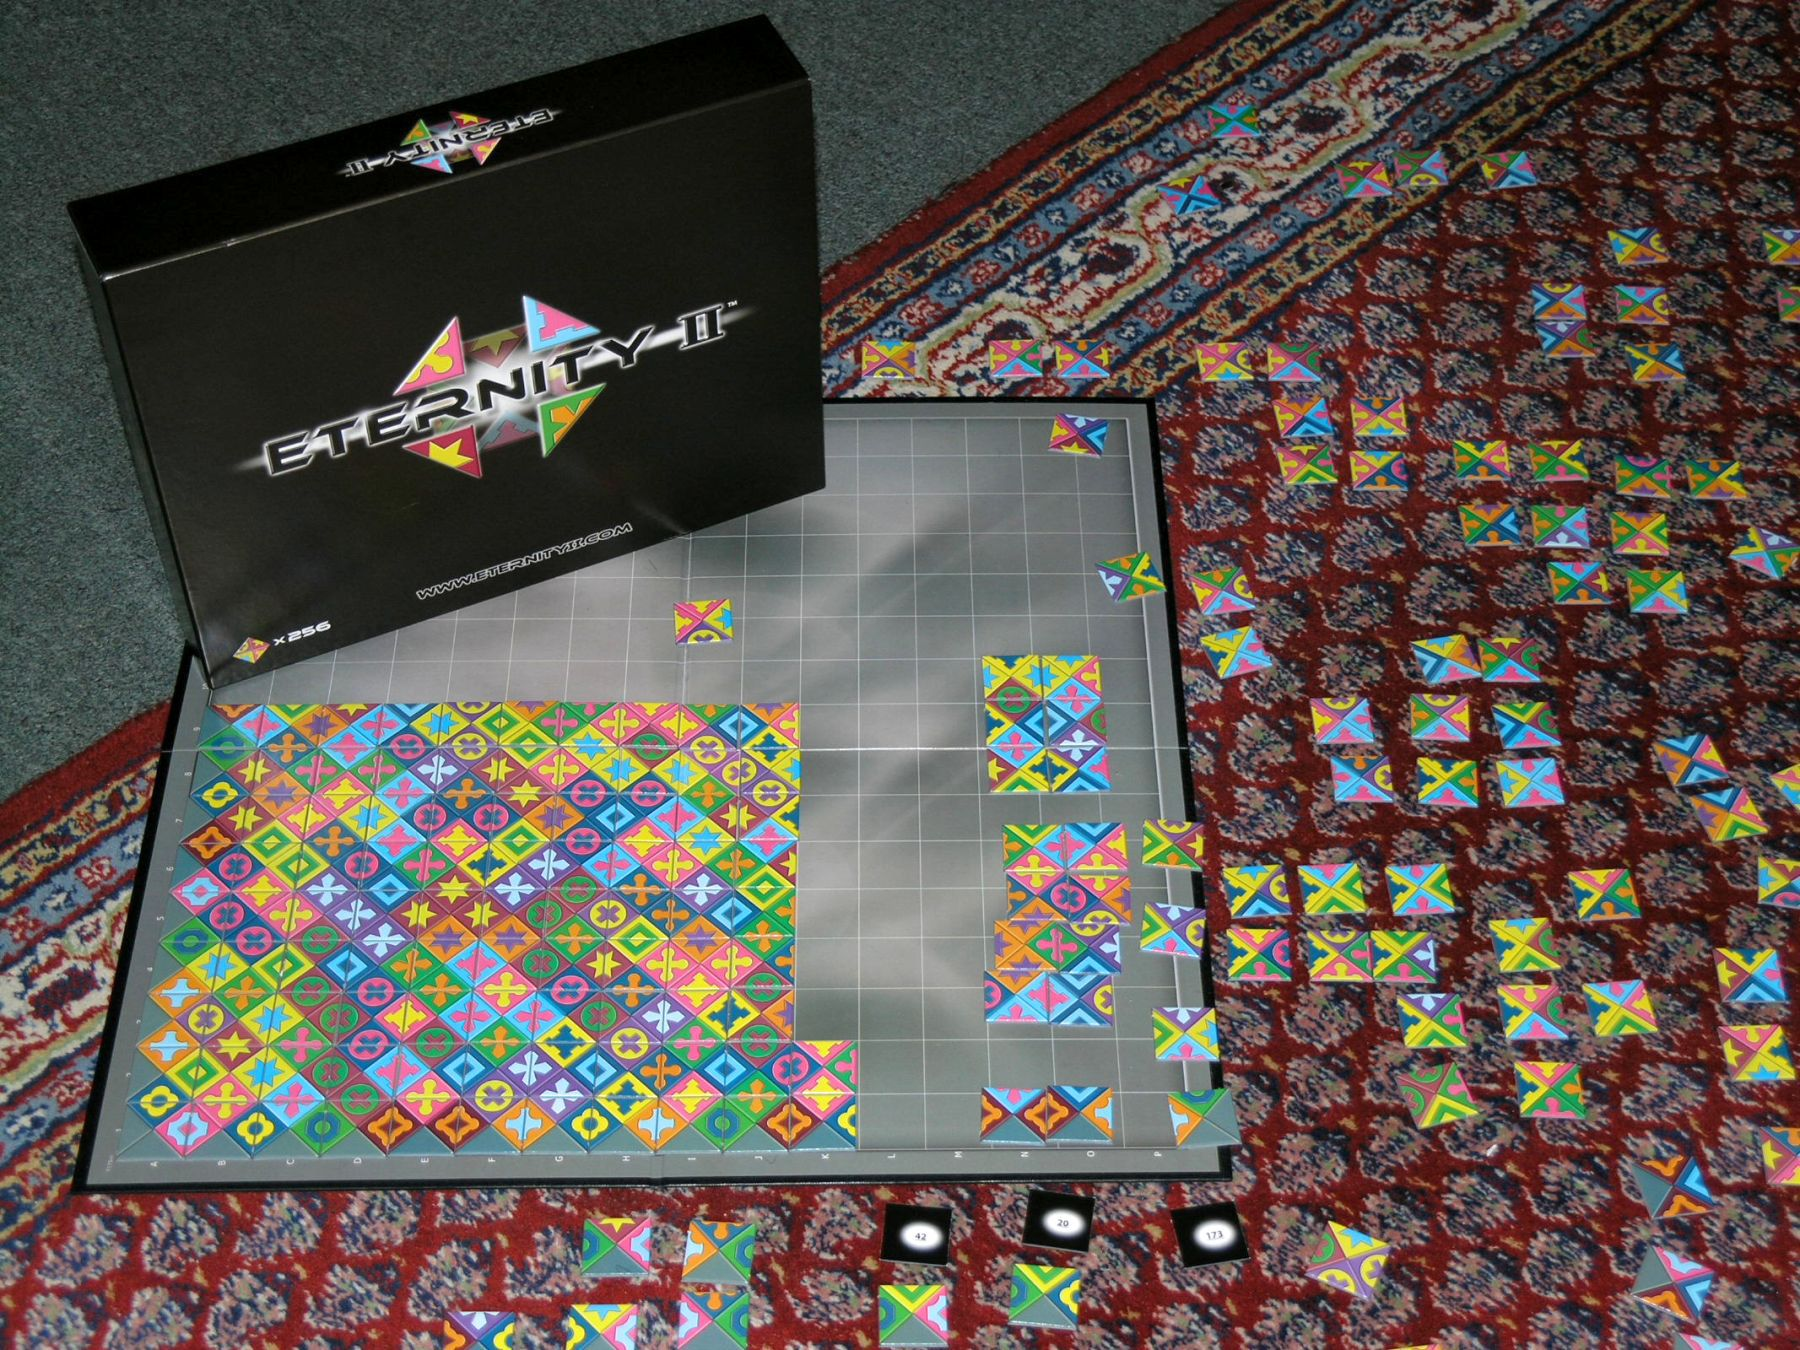
\includegraphics[width=\linewidth]{images/eternity_2.jpg}
		\caption{La boite et les pièces d'Eternity II}
		\label{fig:eternity_2}
	\end{figure}
	
	C'est un puzzle de 16 par 16 qui sort sous le nom d'Eternity II. Ce puzzle est composé de 256 pièces carrés, qui ont chacune 4 faces colorés (ou un demi motif).
	
	Ces pièces peuvent être classés en trois catégories suivant le nombre de faces grises qu'elles possèdent :
	
	\begin{figure}[H]
	   	\minipage{0.32\textwidth}
	   	
\includegraphics[width=\linewidth]{images/piece_coin.png}
	   	\caption{\textbf{pièce de coin :} 2 faces grises}\label{fig:piece_coin}
	   	\endminipage\hfill
	   	\minipage{0.32\textwidth}
	   	
\includegraphics[width=\linewidth]{images/piece_bord.png}
	   	\caption{\textbf{pièce de bord :} 1 faces grise}\label{fig:piece_bord}
	   	\endminipage\hfill
	   	\minipage{0.32\textwidth}
	   	
\includegraphics[width=\linewidth]{images/piece_interieure.png}
	   	\caption{\textbf{pièce d'intérieur :} toutes les faces de couleur}\label{fig:piece_interieure}
	   	\endminipage
	\end{figure}

	Les pièces ne possèdent pas de formes comme dans un puzzle classique. Afin de les faire correspondre l'une avec l'autre, il est nécessaire que les faces adjacentes de chaque pièce voisine soient de la même couleur, dés lors les pièces \enquote{matchent} \ref{fig:matching}.
	
	\begin{figure}[H]
		\centering
		
\includegraphics{images/matching_pieces.png}
		\caption{Deux pièces correctement placés (matchés)}\label{fig:matching}
	\end{figure}
	
	Par conséquent, une pièce peut quasiment être placée n'importe où sur le plateau car son placement dépend des couleurs des pièces d'à côté, de plus, les pièces n'ont pas d'orientation prédéterminés (elles peuvent être rotationnée).
	
	Pour résumer, la plupart des pièces peuvent être posés n'importe où sur le plateau à différentes rotation car la position dépends entièrement des pièces adjacentes posés auparavant. 
	
	Enfin, comme leur nom l'indiquent, les pièces de coins sont les seules à pouvoir être posés dans les coins du plateau, c'est aussi valable pour les pièces de bord qui ne peuvent être placés que sur les bords du plateau, ces deux types de pièces ne peuvent pas être ailleurs car leurs faces grises doit \enquote{matcher} avec les bords du plateau.
	
	
	--- [résumé]
	
	Eternity II est un jeu sorti en 2008 qui repose sur un principe assez simple, c'est un puzzle de 16 par 16 qu'il faut réassembler. Il est composé de 256 pièces carrés, qui ont, sur chaque arête une couleur donnée. [images tt ca tt ca]. Afin de pouvoir assembler le puzzle, il suffit placer les pièces de façon à ce que les faces adjacentes soient de même couleur. Comme un puzzle classique, il y a des pièces de coin et de bord. Ceux-ci sont reconnaissables car ils possèdent une ou deux arêtes grises. Par contre, la où ca devient complexe, c'est qu'une pièce n'as pas une place prédéterminée (comme dans un puzzle), c'est à dire qu'elle peux se situer n'importe où sur le plateau. 
	
	\newpage
	\subsection{Le défi}
	--- [réel]
	
	Malgré le fait que la récompense à expiré le 31 décembre de l'année 2010, le problème et l'enthousiasme qu'a engendré Eternity II ne c'est pas calmé pour autant (enfin si\dots un peu). Car loin d'être juste un jeu avec une importante cagnotte il recel en son c\oe ur des secrets d'une certaine valeur.
	
	En effet, jusqu'à maintenant, personne n'a réussi à résoudre ce puzzle, même pas effleuré la solution, malgré l'aide de supercalculateurs et de nombreux spécialistes, que ce soient des mathématiciens ou des informaticiens.
	
	Pourquoi ? Car derrière ce jeu anodin se cache l'un des plus grand problème du monde actuel : les problèmes NP-difficiles. Ceux-ci sont fait de telle sorte que même ne connaissant leur structure ou fonctionnement, il est pratiquement impossible d'en déduire un algorithme (moyen de résoudre) afin de trouver la solution. Ce type de problème est communément appliqué dans le chiffrement. Car le meilleur moyen de cacher une aiguille (solution) est de la cacher dans gros paquet d'aiguilles, plus le tas est gros, plus on met de temps à la [l'aiguille] trouver.
	
	\begin{exmp}
		Le nombre de combinaisons possibles pour Eternity II s'élève à $10^{545}$, c'est à dire environ $10^{450}$ fois le nombre d'atomes dans l'univers connu (estimé à au plus $10^{80}$) !!! Ca fait un gros tas d'aiguilles !!
	\end{exmp}
		
	--- [résumé]
	
	A ce jour, personne n'a réussi à résoudre ce puzzle (même grâce à l'aide de supercalculateurs) malgré les différentes stratégies mise en place. Pourquoi ? Car derrière ce jeu anodin se cache l'un des plus grand problème du monde actuel : les problèmes NP-difficiles. Ceux-ci sont fait de tel sorte que même en connaissant leur structure ou fonctionnement, il est pratiquement impossible d'en déduire un algorithme de résolution. L'une des solutions les plus fiables à ce jour est de tester tout les cas possible (qui est évidemment très important).
	
	\begin{exmp}
		Le nombre de combinaisons pour Eternity II s'élève à $10^{545}$, c'est à dire environ $10^{450}$ fois le nombre d'atomes dans l'univers connu (estimé à au plus $10^{80}$) !!!
	\end{exmp}
	
	\subsection{Les II lois d'Eternity II}
	
	--- [réel]
	
	Pour rendre Eternity II complexe et combinatoire, il est nécessaire de respecter les deux lois d'Eternity II :
	
	\begin{law}
		\textbf{Chaque pièce est unique}
		
		L'unicité des pièces est indispensable pour complexifier le problème, car sinon, on peux considérer qu'une pièce peux être placée à plusieurs endroits, en fonction du nombre de \enquote{clones} qu'elle possède. Ce qui réduit grandement l'espace de recherche [de la solution].
	\end{law}

	\begin{law}
		\textbf{La quantité de couleurs et de pièces est finement calculée}
		
		En effet, si l'on augmente le nombre de couleurs, on obtient des couplage uniques : une pièce ne peux être couplée qu'avec une autre pièce (ou dans le meilleur des cas limite le couplage des pièces). A l'inverse, si il n'y a pas assez de couleurs, on obtient des doublons, les pièces ne sont plus uniques, ce qui va à l'encontre de la première loi.
		
		Par ailleurs, certaines couleurs sont exclusives aux pièces de coin et de bord, car ceux-ci étant liés en eux mais seulement sur le périmètre extérieur du plateau il est nécessaire d'ajouter des couleurs supplémentaires tenant compte qu'ils n'ont que 2 ou 3 faces disponibles (le reste étant des faces grises).
	\end{law}
	
	
	--- [résumé]
	
	Pour rendre ce problème combinatoire, il est nécessaire de respecter plusieurs conditions.
	
	\begin{description}
		\item[Chaque pièce est unique] l'unicité des pièces est importante, car si une pièce est en double, cela veux dire que la pièce peux être placée à deux endroits différents (ce qui simplifie le problème)
		\item[Le ratio de nombre de couleurs par nombre de pièces est calculé] [joindre graphique tt ca tt ca] : il faut qu'il y ait assez de couleur pour que chaque pièce soit unique, mais pas assez pour que l'on puisse déterminer les pièces adjacentes
		
		\begin{exmp}
			Supposons qu'il y ait trop de couleurs. Cela veux dire qu'une pièce à peu de voisins ( car chaque pièce est unique, par conséquent les couleurs sont distribués uniformément à travers les pièces), si la pièce à très peu de voisins, je peux déduire des groupement de pièces assez facilement.
			
			Donc je simplifie mon problème.
		\end{exmp}		
	\end{description}
	
	\subsection{Etat de l'art}
	
	Un grand nombre de méthodes ont été mis en place afin de résoudre ce problème.
	
	Il serait trop long de présenter et décrire les différents méthodes mise en place car il requièrent une certaine connaissance dans les domaines auxquels ils sont appliqués. Malgré tout, Les différentes approches seront notés ici à titre informatif.
	
	Pour commencer, il existe plusieurs solveurs graphiques afin de pouvoir résoudre le puzzle manuellement ou assisté par l'ordinateur. Certains d'entre eux permettent même l'import export de la progression actuelle.
	
	\begin{itemize}
		\item E2\_manual : \url{https://sourceforge.net/projects/e2manual/}(anglais)
		\item E2Lab : \url{http://eternityii.free.fr/}(anglais)
	\end{itemize}
	
	Ensuite, il existe un très grand nombre de solveurs bruteforce plus au moins rapides. Certains d'entre eux peuvent agréger plusieurs machines afin d'augmenter la puissance de calcul via le réseau.
	
	Ce problème a été abordé de façon très varié au niveau théorique et applicatif.
	
	Par exemple, Eternity à été adopté sous forme de graphe \cite{patey2010eternity} ou de sous forme de contraintes \cite{benoist2008programmation}.
	
	On note aussi un procédé intéressent de résolution grâce à une approche nommée \textbf{SAT} (satisfaisabilité booléenne) s'appuyant sur la logique propositionnelle \cite{cuvillierresolution} \cite{heule2009solving}.
	
	--- [résumé]
	
	Nombreux sont ceux qui ont essayé de résoudre le problème... plusieurs moyens ont été mis en place, grâce au solveur SAT (solveur de satisfiabilité booléenne dont le fonctionnement est assez complexe pour ne pas être abordé ici), par une approche graphe ou encore par bruteforce.
	
	Il est estimé que actuellement, l'approche la plus performante est la résolution par bruteforce, car c'est elle qui est la plus rapide.

	\newpage
	% !TeX root = main.tex
\section{Problématique}

	Le but du stage est donc de déterminer si, malgré les dires, on pourrait trouver une méthode de résolution plus efficace que la bruteforce, qui reposerait sur une grande quantité d'information pré-calculées, cette méthode sera appelée smartforce par la suite.

	Ces informations pré-calculées serviront différentes causes, mais deux objectifs principaux peuvent en être explicités :

	\begin{itemize}
		\item les ouvertures
		\item les finales
	\end{itemize}

	Afin de comprendre le principe des ouvertures et des finales, il est important de pouvoir se représenter un arbre de possibilités où chaque branche de l'arbre est une combinaison spécifique.

	\begin{exmp}
		Prenons pour exemple l'arbre des possibilités d'un lancé de monnaie (en supposant que la monnaie ne tombe pas sur la tranche \cite{murray1993probability}). A chaque étape, deux choix s'offrent à nous :
		\begin{itemize}
			\item la pièce tombe sur pile
			\item la pièce tombe sur face
		\end{itemize}

    Supposons que l'on lance la pièce trois fois. On à donc un arbre ressemblant à ça :

    \begin{figure}[H]
    	\begin{center}
    		\includestandalone[mode=image]{graphics/coin_tree}	
    	\end{center}
    \caption{Arbre de possibilités d'un lancer de monnaie}
    \label{fig:coin_tree}
    \end{figure}

    Grâce à cet arbre, à chaque fois qu'une pièce sera lancée jusqu'à trois fois d'affilés, la combinaison (ou chemin) figurera dans l'arbre.
    
    Chaque n\oe ud de l'arbre possède un sous-arbre (si il est pris comme racine), ce sous-arbre peut être vide.
	\end{exmp}
	
	\begin{note}
		Pour l'arbre de résolution d'EternityII, c'est à peu près la même chose mais l'arbre est bien plus grand. Les n\oe uds de celui-ci ne peuvent pas être prédits (on ne connait que les n\oe uds suivants du chemin emprunté).
	\end{note}

	Cet arbre sera représenté par la suite sous cette forme :
	\begin{figure}[H]
	   	\begin{center}
	   		\includestandalone[mode=image]{graphics/triangle}	
	   	\end{center}
	   	
	   	\caption{Représentation simplifiée d'un arbre de possibilité}
	   	\label{fig:arbre}
	\end{figure}
	 \newpage

	\subsection{Ouvertures}
	
	L'idée est de pré-calculer tous les débuts jusqu'à un certaine profondeur de l'arbre pour ensuite créer des sous-arbres pouvant être parcourus parallèlement ou pondérer les sous-arbres générés pour les classer (par taille, \dots).
	
	\begin{exmp}
		Dans le cas du lancé de monnaie, je sais que le premier lancer, me donne soit pile soit face. En connaissant cela, je peux séparer l'arbre en deux sous-arbres. Cela m'évite de recalculer la première profondeur
		

		
		\begin{figure}[H]
			\minipage{0.49\textwidth}
			\begin{center}
				\includestandalone{graphics/coin_sub_tree_even}
			\end{center}
			\caption{Sous-arbre de pile}\label{fig:sous-arbre-pile}
			\endminipage\hfill
			\minipage{0.49\textwidth}
			\begin{center}
				\includestandalone{graphics/coin_sub_tree_odd}
			\end{center}
			\caption{Sous-arbre de face}\label{fig:sous-arbre-face}
			\endminipage\hfill
		\end{figure}
	\end{exmp}
	
	\begin{rem}
		L'utilité des ouvertures dans un lancé de pièce (de monnaie) est très discutable, mais elle prends son sens lorsque
		
		\begin{itemize}
			\item le calcul de chaque n\oe ud est gourmand
			\item la quantité de n\oe uds est importante
		\end{itemize}  
	\end{rem}
	
	L'arbre des possibilités dans le cas des ouvertures est représenté comme ceci :
	
	\begin{figure}[H]
		\begin{center}
			\includestandalone[mode=image]{graphics/ouvertures}	
		\end{center}
		
		\caption{Représentation simplifiée des ouvertures}
		\label{fig:ouvertures}
	\end{figure}
		
	Le triangle des possibilités est tronqué car le début a déjà été pré-calculé, c'est comme si l'on avait placé tout les sous-arbre côte à côte. Les ouvertures étant stockées sous forme de données, elles sont représentés par un carré.
\newpage

	\subsection{Finales}

	Les finales permettent de prédire si le chemin emprunté dans l'arbre mène à une solution. Par conséquent, toutes les finales possibles sont pré-calculés et stockés sous forme de données.
	
	Grâce à cela, on peux connaître si le chemin choisi (ou combinaison actuelle) est possible sans avoir à finir le chemin en entier.
	
	Les finales sont représentés comme ceci :
	
	\begin{figure}[H]
		\begin{center}
			\includestandalone[mode=image]{graphics/finales}	
		\end{center}
		
		\caption{Représentation simplifiée des finales}
		\label{fig:finales}
	\end{figure}
	\newpage
	
	\subsection{Objectif}
	
	Grâce à l'aide de ces deux approches. on peux donc diminuer drastiquement la quantité de calcul nécessaire en augmentant la quantité de données stockés. Par ailleurs, en adaptant la méthode de résolution on peux aussi réduire la profondeur totale de l'arbre.
	
	Par conséquent, on réduit non seulement ce qui reste à déterminer, mais aussi la taille de l'arbre dans son ensemble.
	
	\begin{figure}[H]
		\minipage[b]{0.49\textwidth}
		\begin{center}
			\includestandalone[mode=image]{graphics/ouvertures_finales}	
		\end{center}
		\caption{Représentation de la fusion des ouvertures et des finales}
		\label{fig:ouvertures_finales}
		\endminipage\hfill
		\minipage[b]{0.49\textwidth}
		\begin{center}
			\includestandalone[mode=image]{graphics/objectif}	
		\end{center}
		\caption{Représentation simplifiée de l'objectif comprenant les ouvertures, les finales et les données}\label{fig:objectif}
		\endminipage\hfill
	\end{figure}
	
	Par la suite, en supposant que l'emploi des données pré-calculées est longue et fastidieuse, le but sera d'aussi utiliser des technologies avancées afin d'accélérer la résolution.

	\section{Approche}

	Dans cette partie, nous expliquerons quels sont les différents outils et stratégies mis en place pour permettre la résolution du problème.
	Dans un premier temps nous avons eu besoin de mettre en place une valeur étalon, qui nous permet de savoir si les differentes méthodes de smartforce sont bonnes ou pas. Cette valeur étalon est un programme de bruteforce qui nous fournit le nombre total de noeuds, le nombre de solution, le nombre de noeuds à la premiere solution et les tous les timers correspondant.

	\subsection{Bruteforce}

	Afin de pouvoir partir sur de bonnes bases, plusieurs différents méthodes de parcours (quel chemin prendre pour résoudre mon plateau) ont été utilisé, afin de voir quel parcours est le plus performant pour la résolution brute. En sachant que le nombre de noeuds/sec est la même, l'unité de mesure est le nombre de noeuds.

	Les differents types de parcours sont :

	\begin{description}
		\item[rowscan] on pose les pieces en lignes horizontales sur le plateau
		\item[diagonal] on pose les pieces en diagonal
		\item[spiral in] on dispose les pièces en spirale en partant de l'exterieur [image]
		\item[spiral out] idem que spiral in mais en partant de l'interieur vers l'exterieur
	\end{description}

	Ces différents types de parcours ont été testés sur plusieurs instances de taille variable.

	\subsection{Smartforce}

	Une fois la valeur étalon fixée, il est maintenant facile de mettre en place un autre approche du problème qui à pour principe de cumuler une grande quantité de donnée pour faire face au nombre exponentiel de possibilités.

	Les différents types de données (nommés modèles) sont comme différents points de vues du problème. Ils sont plus ou moins utiles, mais la force réside dans leur union. Mais surtout, ils permettent de mettre en place le concept d'ouvertures et finales.

	\subsubsection{CaPi}

	L'approche CaPi (abbréviation de Cases/pieces) est l'approche la plus naive, elle permet de définir quelle piece peut être placée sur telle case et inversement, quelle case peux avoir telle piece.

	Cette approche est l'interaction la plus basique de notre problème. C'est aussi celle-ci qui est utilisée en bruteforce.

	\subsubsection{BoCo}

	L'approche BoCo (Bordure/Couleur) est bien plus fine : si l'on connait quelle piece est sur telle case, on sait quelle couleur peux se placer sur telle bordure [de la case]. Elle permet d'implémenter un système de mis à jour bien plus performant car ne nombre de couleurs est bien plus petit que le nombre de pièces.

	\begin{exmp}
		Si une couleur disparait, alors tt les pièces ayant cette couleur ne peuvent plus être placés à cette case, par conséquent, les autres bords de la case ont (probablement) des couleurs qui disparaissent aussi (propagation de la disparition).
	\end{exmp}

	\subsubsection{Corolles}

	Grace aux visions CaPi et BoCo, il est possible de pré-calculer des zones du plateau nommés corolles, ceux-ci contiennent tous les cas possibles dans cette zone donnée.

	Le nombre de cas possible étant très important, il est nécessaire de le classer. Les corolles peuvent êtres identifiés grâce à plusieurs critères.

	\begin{itemize}
		\item taille du plateau
		\item l'orientation de la corolle
		\item La pièce (et sa rotation) à l'origine de la corolle
		\item La case à l'origine de la corolle
		\item La taille de la corolle
	\end{itemize}

	\paragraph{position et orientation des corolles}

	\subsubsection{BoCoDiag}

	\section{Application}

	\section{Resultats}

	\section{Manuel d'utilisation}

	\section{Manuel Technique}


	\bibliographystyle{plain-fr}
	\bibliography{biblio}

\end{document}
